
%% bare_conf.tex
%% V1.3
%% 2007/01/11
%% by Michael Shell
%% See:
%% http://www.michaelshell.org/
%% for current contact information.
%%
%% This is a skeleton file demonstrating the use of IEEEtran.cls
%% (requires IEEEtran.cls version 1.7 or later) with an IEEE conference paper.
%%
%% Support sites:
%% http://www.michaelshell.org/tex/ieeetran/
%% http://www.ctan.org/tex-archive/macros/latex/contrib/IEEEtran/
%% and
%% http://www.ieee.org/

%%*************************************************************************
%% Legal Notice:
%% This code is offered as-is without any warranty either expressed or
%% implied; without even the implied warranty of MERCHANTABILITY or
%% FITNESS FOR A PARTICULAR PURPOSE! 
%% User assumes all risk.
%% In no event shall IEEE or any contributor to this code be liable for
%% any damages or losses, including, but not limited to, incidental,
%% consequential, or any other damages, resulting from the use or misuse
%% of any information contained here.
%%
%% All comments are the opinions of their respective authors and are not
%% necessarily endorsed by the IEEE.
%%
%% This work is distributed under the LaTeX Project Public License (LPPL)
%% ( http://www.latex-project.org/ ) version 1.3, and may be freely used,
%% distributed and modified. A copy of the LPPL, version 1.3, is included
%% in the base LaTeX documentation of all distributions of LaTeX released
%% 2003/12/01 or later.
%% Retain all contribution notices and credits.
%% ** Modified files should be clearly indicated as such, including  **
%% ** renaming them and changing author support contact information. **
%%
%% File list of work: IEEEtran.cls, IEEEtran_HOWTO.pdf, bare_adv.tex,
%%                    bare_conf.tex, bare_jrnl.tex, bare_jrnl_compsoc.tex
%%*************************************************************************
%
\documentclass[conference]{./IEEEtran}

\usepackage{graphicx}
\usepackage{pgfplots}
\usepackage{tikz}

\begin{filecontents}{comp.dat}
Coord Title Lowest Highest
1 {\rotatebox{45}{None}}		          0.017 0.031 
2 {\rotatebox{45}{Sleep mode}}        0.014 0.029
3 {\rotatebox{45}{PRR}}		            0.017 0.029
4 {\rotatebox{45}{Pull Up Resistors}}	0.009 0.022
5 {\rotatebox{45}{All}}		            0.004 0.019

\end{filecontents}

\begin{document}
%
% paper title
% can use linebreaks \\ within to get better formatting as desired
\title{ADXL345 Knock Pattern Sensor}


% author names and affiliations
% use a multiple column layout for up to three different
% affiliations
\author{\IEEEauthorblockN{Allison Pearce}
\IEEEauthorblockA{St. Edmund's College\\ 
ap819@cam.ac.uk}
}

\maketitle


\section{Introduction}
% objective
% something about passwords sucking
% usefulness of knock patterns
% prior work? probably wouldn't hurt to cite something
This paper describes a low-power knock pattern sensor built using an Atmel ATmega 644P microcontroller \cite{atmega644p} and an ADXL345 triple axis accelerometer \cite{devices2011adxl345}. Knock pattern sensors have a number of useful applications. Shock sensors are often used to detect forcible entry into roadside telecommunications cabinets, and when a knock sensor is present, authorized personnel can enter a tap code to override the alarm. Knock patterns can also be used as an unlocking mechanism for a door or safe. Tap authentication has been investigated as a replacement for passwords in mobile devices, indicating that tap authentication is comparable to industry standards for security and usability with the added advantage of being inconspicuous \cite{marques}. Tapping wireless devices together can also form part of a protocol for communication and information transfer \cite{thorn}. For example, users can tap two phones together to share an image from one to the other.

The goal of this project was to make a functional knock pattern sensor that could compare a reasonably complex knock pattern to a previously recorded pattern. This required sensitive tap detection with minimal false positives and a method of representing and comparing knock patterns. The device also needed to be low power and user friendly. 

\section{Preparation}
% Any assumptions made, which devices used and why, is there enough storage capacity for example.
\subsection{Device Selection}
This project required a microcontroller and a sensor to perform knock detection. I selected the Ateml ATmega 644P for the microcontroller because it is easy to use and supports the SPI communication needed for the accelerometer. It has several features for reducing power use. The system's storage requirements were low, and the ATmega 644P's memory was more than sufficient. I was also familiar with it from previous P31 practical work. 

The ADXL345 triple axis accelerometer was chosen as the knock sensor for its sensitivity and ease of use. Alternatives included shock sensors and other types of accelerometers. An accelerometer was preferred to a shock sensor because previous implementations of knock pattern sensors reported that shock sensors were difficult to interpret. Compared to other accelerometers, the ADXL345 provides several unique and advantageous features. Chief among these is its built-in tap detection function. Taps are defined by several parameters that can be used to tune the sensitivity of the knock sensor, and detected taps can trigger an interrupt in the microcontroller. The ADXL345 is a digital accelerometer that uses SPI or I$^2$C to communicate with the microcontroller. It has one of the lowest accelerometer power requirements. The ADXL345 also provides programmable power modes than can be used to further reduce power consumption.  


\section{Implementation}
% mention that you used the starter code
% especially talk about what was done to reduce power consumption
\subsection{System Overview}
The device has two modes of operation, one for recording passcodes and one for comparing input knock patterns to the stored pattern. The device is initialized in recording mode. The user knocks the pattern, and a green LED flashes as each knock is registered. After three seconds of inactivity, the recording period times out, the red LED flashes the pattern back to the user for verification, and the device enters listening mode. In listening mode, the device sleeps until interrupted by a knock. It will record any subsequent knocks until three seconds pass without activity. Again, the green LED flashes with each tap. It then compares the new pattern to the previously recorded pattern. A green LED flashes if the pattern is correct, otherwise a red LED flashes. To record a new pattern, the user presses the button switch until the LEDs flash in a red-green-red pattern. 

\begin{figure*}
\centering
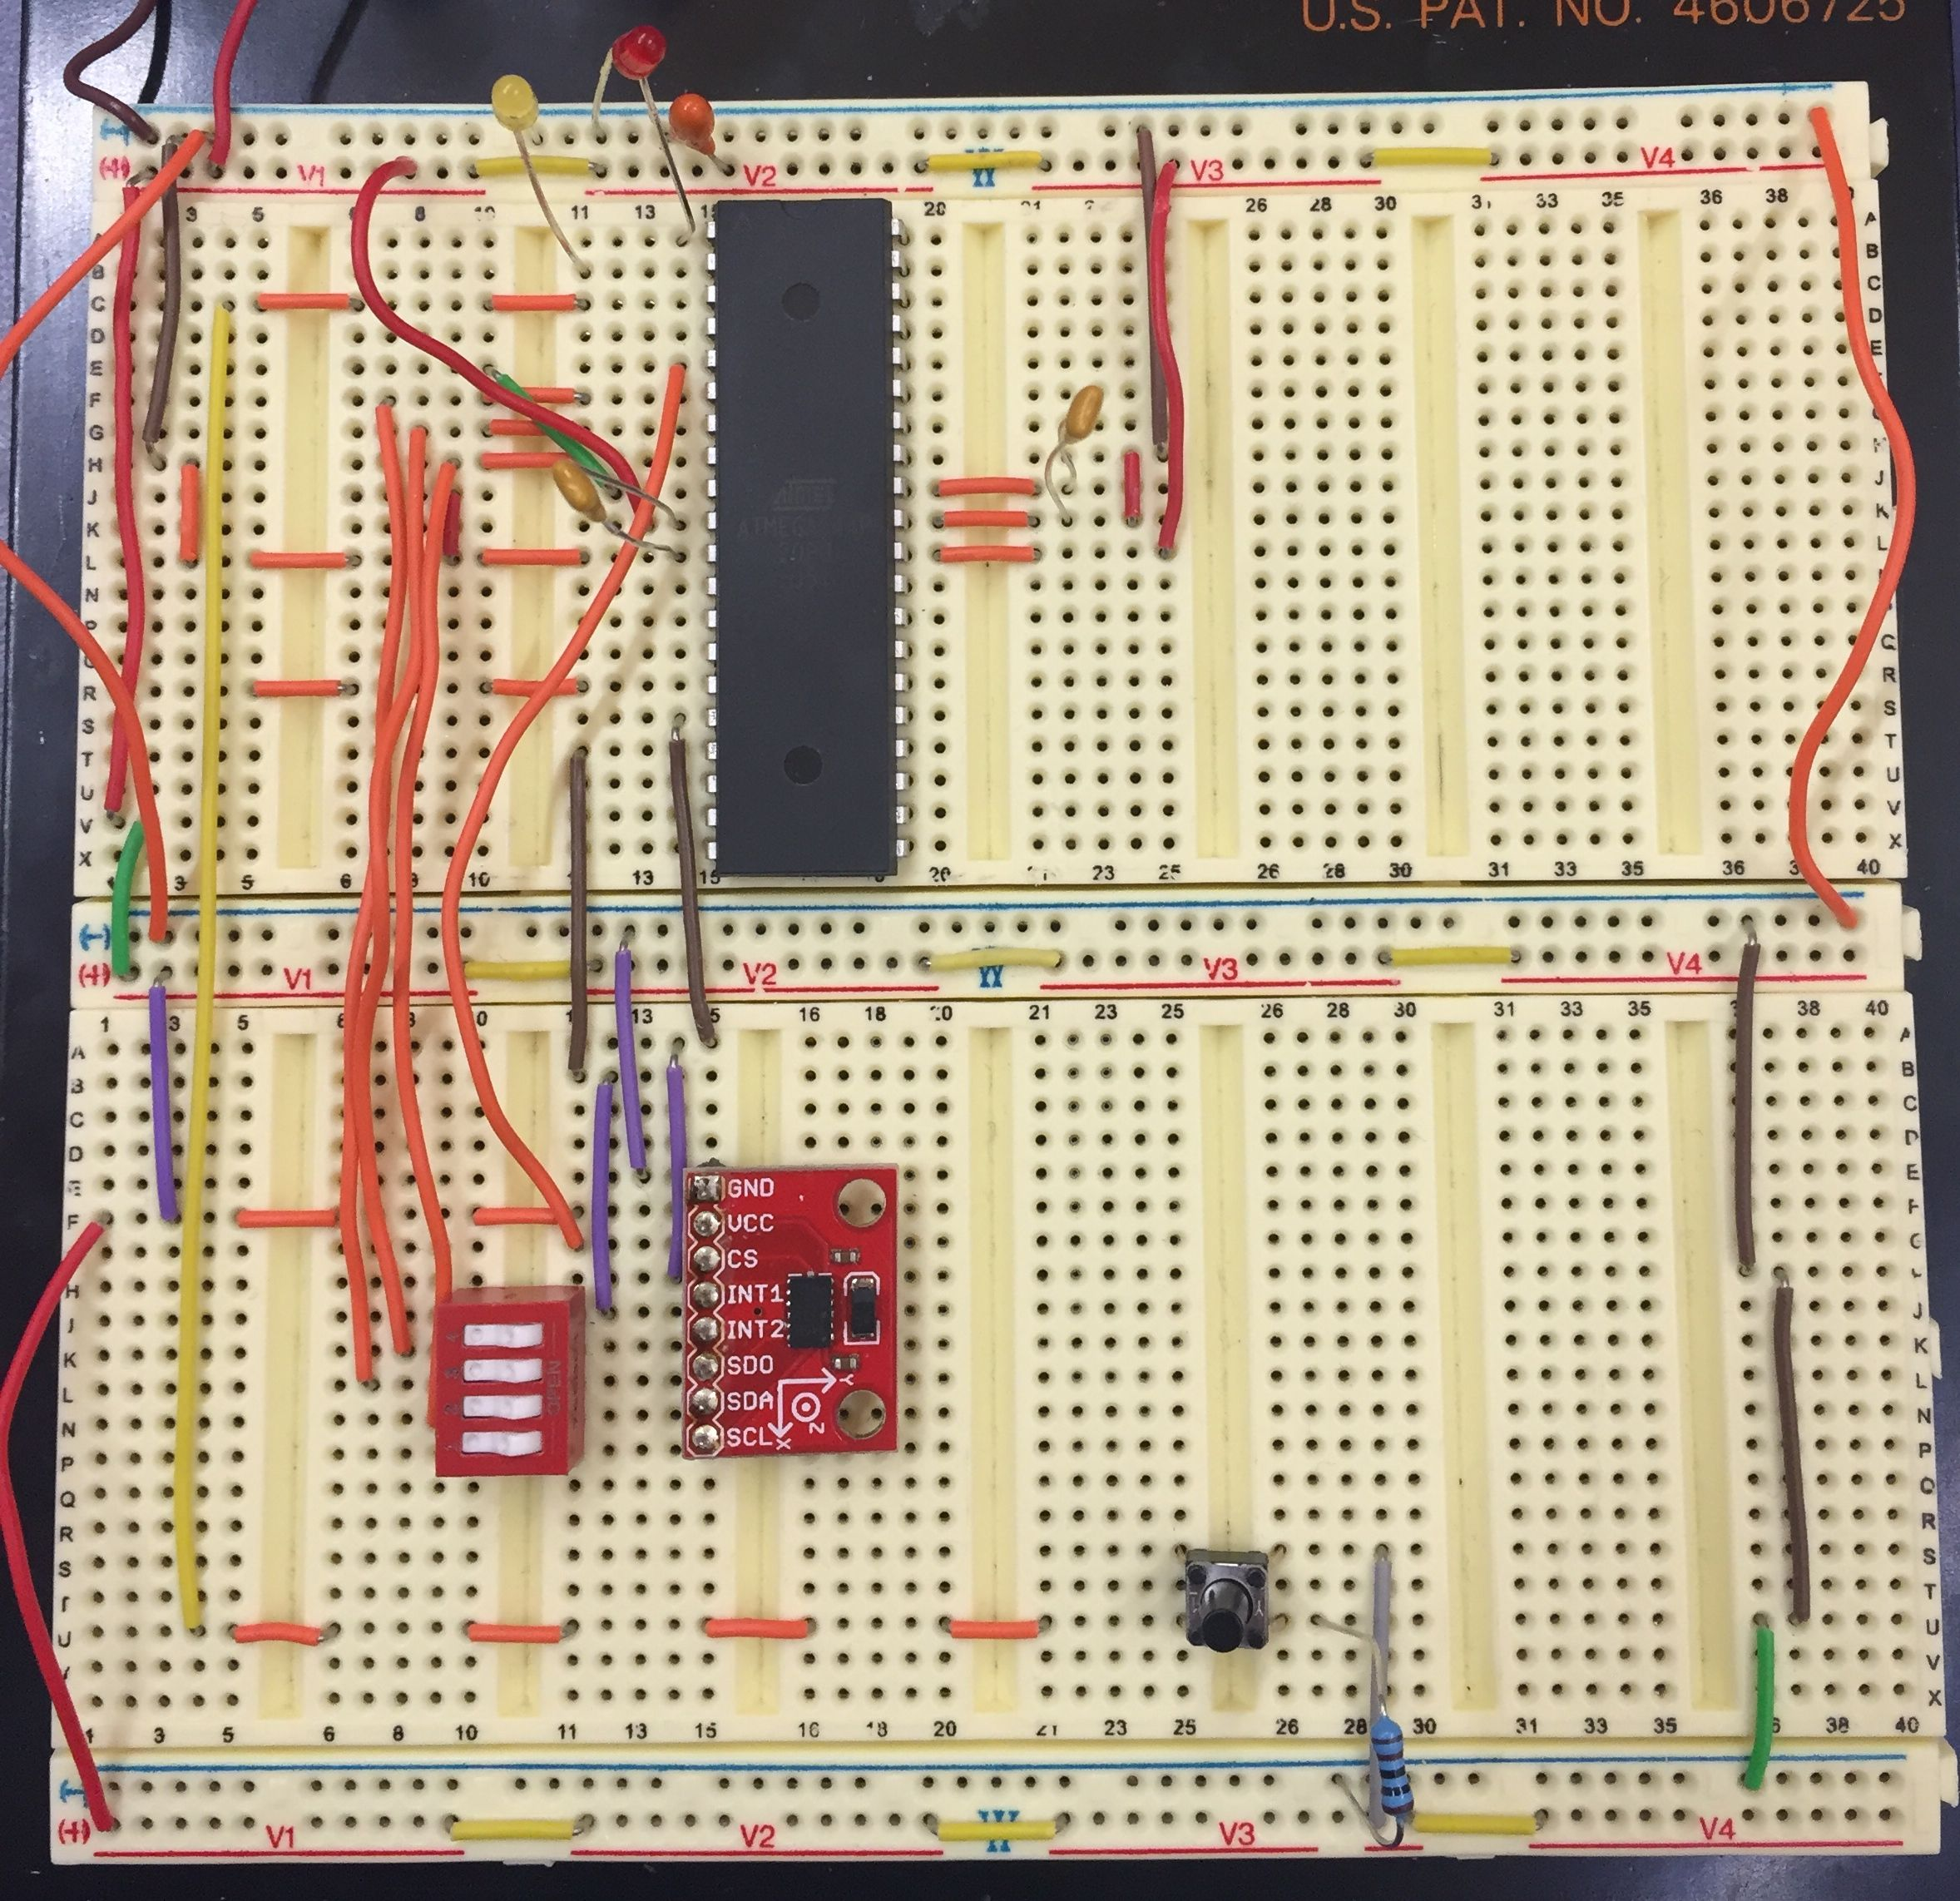
\includegraphics[width=6in]{wires.jpg}
\caption{Connection of components on prototyping board}
\label{wires}
\end{figure*}

\subsection{Hardware}
In addition to the microcontroller and accelerometer, this project required a 5V 100mA power supply, a prototyping board, wires, a programming cable, a four-panel switch, two LEDs, a 1K Ohm resistor, and a button switch. The resistor was used to pull down the button. The four-panel switch was necessary because the accelerometer communicates with the microcontroller over SPI, which uses the same pins (MOSI, MISO, SCK) as the programmer. The microcontroller, accelerometer, and other components were connected as shown in Figure 1.  

\subsection{Software}
% TODO actually read the code; could be more stuff there
The C program executed by the microcontroller consists of several initialization functions, a simple main loop, interrupt handlers, functions to record and compare knock patterns, and functions for communicating with the user via LED flashes. Some of the functions for communicating with the ADXL345 were taken from an example provided on the P31 website.

The initialization functions establish the communication method between the ATmega 644P and the accelerometer, set values for the tap detection parameters and other ADXL345 registers, set parameters for the timer, and enable interrupts. The two most important parameters for tap detection are the tap threshold and the window. The tap threshold determines the minimum acceleration value that is considered a tap, and the window is the maximum time that the acceleration can remain above the threshold. Adjusting these parameters makes the system more or less sensitive to knocks. The other ADXL345 registers that were set and their values are described in Table I.

\begin{table}
% increase table row spacing, adjust to taste
\renewcommand{\arraystretch}{1.3}
\caption{ADXL345 Registers}
\label{table_regs}
\centering
\begin{tabular}{p{2cm}p{4cm}p{1cm}}
\hline
Register & Description & Value\\
\hline
\texttt{THRESH\_TAP} & Minimum acceleration value for taps. Scale factor 62.5$mg$/LSB& 70\\
\texttt{DUR} & Maximum time event can be above threshold to be considered a tap. Scale factor 625$\mu$s/LSB& 16\\
\texttt{LATENT} & For double tap detection. Set to 0 to disable double taps. & 0\\
\texttt{WINDOW} & For double tap detection. Set to 0 to disable double taps. & 0\\
\texttt{TAP\_AXES} & Which axes to use in tap detection. & 0x07\\
\texttt{INT\_ENABLE} & Which interrupts to enable & 0x40\\
\texttt{INT\_MAP} & Map interrupts to microcontroller pins & 0x40 \\
\hline
\end{tabular}
\end{table}


The bulk of the work in the software is triggered from the tap interrupt. Upon receiving the first tap after a period of inactivity, the tap interrupt starts the ATmega 644P's built-in 16-bit timer. Subsequent tap interrupts cause the timer value to be recorded and then clear and restart the timer. A timer interrupt is used to prevent overflow errors in the timer's counter. The timer interrupt is also responsible for calling the appropriate function after three seconds of inactivity: in record mode, it flashes the pattern back to the user, and in verify mode, it compares the input pattern to the recorded pattern and flashes the green or red LED depending on if it was correct.

Knock patterns are defined by the intervals between taps and stored as arrays of integers. When comparing patterns, the new pattern is immediately invalidated if it has a different number of knocks than the code pattern. The new pattern is accepted if it has the same number of taps as the code and each interval is within an acceptable range of the code's interval for that position in the sequence. The range can be changed to tune the sensitivity of the device, but 20ms was determined to be a reasonable default.

The main loop checks to see if a button press has occurred, in which case the mode (record or verify) is toggled. If not, it sets the sleep mode and puts the device to sleep. The full program is included in the Appendix.

One optional feature of the ADXL345 that was disabled in software is double tap detection. It is possible to make a distinction between single taps and double taps by defining additional parameters and flipping bits in the appropriate registers. Handling single and double taps differently offered no significant advantages for distinguishing different knock patterns, but it would have increased the complexity of how knock patterns are stored and compared. 


\subsection{Power Concerns}
Low power consumption was a primary goal of the system achieved through a combination of power reduction strategies. The microcontroller enters ADC noise reduction sleep mode whenever three seconds pass without a knock interrupt. This sleep mode provided the greatest possible power reduction while still allowing the microcontroller to respond to knock interrupts. The accelerometer operates in a power saving mode, with all unnecessary functions turned off in the Power Reduction Register (PRR). TWI, Timer/Counter2, Timer/Counter0, USART1, and USART0 were disabled. Timer/Counter1 and SPI remained on because they were necessary for knock timing and communication with the accelerometer. Another simple strategy that yielded a huge power reduction was adding pull-up resistors on all inputs to prevent them from floating. Though the ADXL345 offers a sleep mode, it was not used because it interfered with tap detection and triggering interrupts in the microcontroller. 

\subsection{Challenges}
A difficult step early in the development process was configuring tap detection on the ADXL345. Most of the process is easy to follow, but I did not initially realize that the \texttt{INT\_SOURCE} register had to be read in the main loop in order for the tap interrupt to fire. Configuring all of the values for the different tap detection registers also required a reasonable amount of experimentation. 

Another step that was less straightforward than expected was determining the proper sleep mode. Based on the documentation for the ATmega 644P and the ADXL345, I expected all of the 644P's sleep modes to work because the INT1 interrupt should be able to wake the microcontroller in all of them. In practice, however, I found that tap interrupts did not wake the microcontroller unless I used ADC noise reduction sleep mode. 

Finally, the use of the four-panel switch to allow the accelerometer and programmer to communicate was a technique I had not encountered before, but thanks to the teaching staff, that problem was solved quickly.

\section{Evaluation}
The goal of the project was to make a low-power knock pattern sensor that was accurate and easy to use. All aspects of this goal were accomplished. 

\subsection{Power Consumption}
% is there a way to compute life of a battery or something based on this
% computing something would probably make me look good
Before any measures were taken to reduce power consumption, the device drew between 0.017mA when idle and 0.031mA when flashing the LEDs. The combination of all power saving strategies reduced these values to 0.004mA and 0.019 mA, respectively. The power savings achieved for each method in isolation are shown in Figure 2.
 \begin{figure}
 \begin{tikzpicture} 
 \begin{axis}[ 
     xtick={1,...,5},
     xticklabels from table = {comp.dat}{Title},
     xtick align=inside,
     every axis x label/.style={at={(ticklabel cs:0.5)},anchor=north east},
     ylabel=Power (mA),
     every axis y label/.style={at={(ticklabel cs:0.5)},rotate=90,anchor=near ticklabel}
 ] 

 \addplot table [ 
     x=Coord,
     y=Lowest
 ] {comp.dat} ;
 \addlegendentry{\small Idle (min)}

 \addplot table [ 
     x=Coord,
     y=Highest
 ] {comp.dat} ;
 \addlegendentry{\small LEDs on (max)}

 \end{axis} 
 \end{tikzpicture} 
 \label{comparison}
 \caption{Power use for different power saving techniques. The red line represents maximum current, when the LEDs were on, and the blue line is minimum current use, when idling between taps.}

 \end{figure}

\subsection{Accuracy}
%TODO talk about how this affects security as well
The accuracy of the device can be affected to some degree by manipulating the sensitivity of the knock sensor. This is achieved by changing the tap threshold, tap window, and the size of the window used to compare knock intervals. A less sensitive knock sensor would register fewer false positive knocks and might perform better in a noisy environment, but it would require the user to be more deliberate about knocking, because lighter taps would not register. This might make it more challenging to input certain types of knock patterns. A more sensitive sensor, on the other hand, might interpret an accidental hand slip as a knock. Therefore it is better for accuracy if the user is aware of the device's settings and how they affect the expectations for knocking. 

Using the default settings from Table I, the device was tested extensively and there were no false positives or false negatives due to the device's error. Human inability to tap in the same pattern multiple times, especially after tapping several intentionally incorrect patterns, was the primary source of error in testing. I also experimented with one user recording the passcode and another user attempting to enter it. Again, the device performed perfectly when the humans involved did not make mistakes. 

\subsection{Ease of Use}
The device was not intended to be a complex system, and it provides all the functionality and feedback required with just one button, two LEDs, and the knock sensor. Resetting the code is a simple process, requiring only a button press and demonstration of the new pattern. The meanings of the various LED flashes are intuitive (green flashes to register knocks, red to replay the pattern, green or red flashes when reporting whether the pattern was correct). 

\section{Future Work}
% how it could be improved, applications
The sensor described in this paper provides all the functionality needed to record and detect knock patterns, but several more sophisticated features could be added. One useful extension would be the ability to store multiple patterns in different categories. This would be useful if the sensor was used to open a door, for example. The owner of the building could have a master pattern and the option to add a one-time passcode for a contractor or a passcode that expires after a set time to be used for guests coming to a party. Other extensions of password modules could also apply, such as providing hints if the user forgets the code. A more sophisticated user interface could be created by adding an LCD screen and a keypad for user inputs other than knock patterns. However, these enhancements would significantly increase the memory and power requirements. Future work could also include incorporating the sensor with an application---attaching it to a servo-based locking mechanism and using it to unlock a door, or integrating it with a laptop or phone to replace the login password. 

\section{Summary}
I implemented a low-power knock pattern sensor that is simple to use and adaptable to a variety of applications. The system was built using an Amtega 644P microcontroller and an ADXL345 triple axis accelerometer. The device is highly accurate and the level of sensitivity can be customized to increase security or to reduce interference from noisy environments. The ADXL345 was an excellent choice for the knock sensor, especially because it provides an easily configured tap detection function. The code for storing and comparing knock patterns was both simple and effective, and did not seem to limit the complexity of knock patterns that could be recorded and verified. This project helped me learn more about microcontrollers, circuits, and their debugging strategies. 

\bibliographystyle{plain}
\bibliography{proj}


% that's all folks
\end{document}



% What DIDN'T work? Where did I get stuck/spend lots of time debugging? 
% Alternatives considered but not used
% software
%   store patterns differently
% hardware 
%   microcontroller, shock sensor
% overall system 
%   more buttons, switches, lights, junk
% add some kind of "challenges" section?
% TODO Fix the references for the tables


% challenges
% figuring out tap detection/making all that jazz work
% figuring out which power modes would work
% 
